\section*{Chapter 4}

\subsection*{Exercise 4.1}

\subsubsection*{Solution:}
In Example 4.1, if $\pi$ is the equiprobable random policy, what is $q_\pi(11, \text{down})$?
What is $q_\pi(7, \text{down})$?

\[
q_\pi(11, \text{down}) = r + v_\pi(\text{end state}) = -1 + 0 = -1
\]

\[
q_\pi(7, \text{down}) = r + v_\pi(11) = -1 - 14 = -15
\]


\subsection*{Exercise 4.2}
In Example 4.1, suppose a new state 15 is added to the gridworld just below
state 13, and its actions, left, up, right, and down, take the agent to states 12, 13, 14,
and 15, respectively. Assume that the transitions from the original states are unchanged.
What, then, is $v_\pi(15)$ for the equiprobable random policy? Now suppose the dynamics of
state 13 are also changed, such that action down from state 13 takes the agent to the new
state 15. What is $v_\pi(15)$ for the equiprobable random policy in this case?

\subsubsection*{Solution:}
First case:
\[
v_\pi(15) = -1 + 0.25(v_\pi(12) + v_\pi(13) + v_\pi(14) + v_\pi(15))
\]

\[
v_\pi(15) = -\frac{4}{3} + \frac{1}{3}(v_\pi(12) + v_\pi(13) + v_\pi(14) ) = -\frac{4}{3} + \frac{1}{3}(-22 - 20 - 14) = -20
\]

Second case:

Using the iterative method with $v_\pi^1(15) = -20$.
\begin{align*}
v_\pi^1(13) &= -1 + 0.25(v_\pi(12) + v_\pi(9) + v_\pi(14) + v_\pi(15)) \\
&= -1 + 0.25(-22 - 20 - 14 - 20) = -20
\end{align*}

The $v(s)$ values didn't change, so the iterative algorithm can terminate here, $v_\pi(15) = -20$.

\subsection*{Exercise 4.3}
What are the equations analogous to (4.3), (4.4), and (4.5), but for action-
value functions instead of state-value functions?

\subsubsection*{Solution:}

\begin{align*}
    q_\pi(s, a) &= \mathbb{E} \left[R_{t+1} + \gamma \sum_{a'} \pi(a' \mid S_{t+1}) q_\pi(S_{t+1}, a') \middle| S_t = s, A_t = a \right] \\
    &= \sum_{s',r} p(s', r \mid s, a) \left(r + \gamma \sum_{a'} \pi(a'\mid s') q_\pi(s', a') \right)
\end{align*}

\[
    q_{k+1}(s, a) = \sum_{s',r} p(s', r \mid s, a) \left(r + \gamma \sum_{a'} \pi(a' \mid s') q_{k}(s', a') \right) 
\]

\subsection*{Exercise 4.4}
The policy iteration algorithm on page 80 has a subtle bug in that it may
never terminate if the policy continually switches between two or more policies that are
equally good. This is okay for pedagogy, but not for actual use. Modify the pseudocode
so that convergence is guaranteed.

\subsubsection*{Solution:}

Instead of 
\[
    \pi(s) \leftarrow \argmax_a \sum_{s',r} p(s',r \mid s,a)[r + \gamma V(s')]
\]

Use:

\[
    \pi(s) \leftarrow \min\{ a \in \argmax_a \sum_{s',r} p(s',r \mid s,a)[r + \gamma V(s')] \}
\]

This way if there are multiple policies that are equally good, the agent always chooses the action with the lowest value. We could also check if $q_\pi(s,\pi(s)) == q_\pi(s,a)$.

\subsection*{Exercise 4.5}
How would policy iteration be defined for action values? Give a complete
algorithm for computing $q_*$, analogous to that on page 80 for computing $v_*$. Please pay
special attention to this exercise, because the ideas involved will be used throughout the
rest of the book.

\subsubsection*{Solution:}
\fbox{
\begin{minipage}{0.95\textwidth}
\footnotesize 
\begin{enumerate}
    \item \textbf{Initialization}\\
    $Q(s,a) \in \mathbb{R}$ and $\pi(s) \in A(s)$ arbitrarily for all $s \in S$; $Q(\text{terminal}, a) \doteq 0$

    \item \textbf{Policy Evaluation}\\
    Loop: 
    \begin{itemize}
        \item[] $\Delta \leftarrow 0$
        \item[] Loop for each $s \in S$:
        \begin{itemize}
            \item[] Loop for each $a \in A(s)$:
            \begin{itemize}
                \item[] $q \leftarrow Q(s,a)$
                \item[] $Q(s,a) \leftarrow \sum_{s',r} p(s', r \mid s, a) [r + \gamma Q(s', \pi(s'))]$
                \item[] $\Delta \leftarrow \max(\Delta, |q - Q(s,a)|)$
            \end{itemize}
        \end{itemize}
    \end{itemize}
    until $\Delta < \theta$ (a small positive number determining the accuracy of estimation)

    \item \textbf{Policy Improvement}
    \begin{itemize}
        \item[] $\textit{policy-stable} \leftarrow \textit{true}$
        \item[] For each $s \in S$:
        \begin{itemize}
            \item[] $\textit{old-action} \leftarrow \pi(s)$
            \item[] $\pi(s) \leftarrow \argmax_a Q(s,a) $
            \item[] If $\textit{old-action} \neq \pi(s)$, then $\textit{policy-stable} \leftarrow \textit{false}$
        \end{itemize}
    \end{itemize}
    If $\textit{policy-stable}$, then stop and return $Q \approx q_*$ and $\pi \approx \pi_*$; else go to 2
\end{enumerate}
\end{minipage}
}

\subsection*{Exercise 4.6}
Suppose you are restricted to considering only policies that are $\varepsilon$-soft,
meaning that the probability of selecting each action in each state, $s$, is at least $\varepsilon/|A(s)|$.
Describe qualitatively the changes that would be required in each of the steps 3, 2, and 1,
in that order, of the policy iteration algorithm for $v_*$ on page 80.

\subsubsection*{Solution:}

\begin{enumerate}
    \item $\pi(a \mid s) = 1/|A(s)|$
    \item $V(s) \leftarrow \sum_a \pi(a \mid s) \sum_{s',r} p(s',r \mid s, a) (r + \gamma V(s'))$
    \item \footnotesize $
    \pi(a \mid s) =
        \begin{cases}
            1-\varepsilon + \frac{\varepsilon}{|A(s)|},  & \text{if } a = \arg \max_a \sum_{s',r} p(s', r \mid s, a) [r + \gamma V(s')]\\
            \frac{\varepsilon}{|A(s)|},  & \text{else}
        \end{cases}
    $
\end{enumerate}

\subsection*{Exercise 4.7 (programming)}
Write a program for policy iteration and re-solve Jack's car
rental problem with the following changes. One of Jack's employees at the first location
rides a bus home each night and lives near the second location. She is happy to shuttle
one car to the second location for free. Each additional car still costs \$2, as do all cars
moved in the other direction. In addition, Jack has limited parking space at each location.
If more than 10 cars are kept overnight at a location (after any moving of cars), then an
additional cost of \$4 must be incurred to use a second parking lot (independent of how
many cars are kept there). These sorts of nonlinearities and arbitrary dynamics often
occur in real problems and cannot easily be handled by optimization methods other than
dynamic programming. To check your program, first replicate the results given for the
original problem.

\subsubsection*{Solution:}

See the notebooks.

\begin{figure}[H]
    \centering
    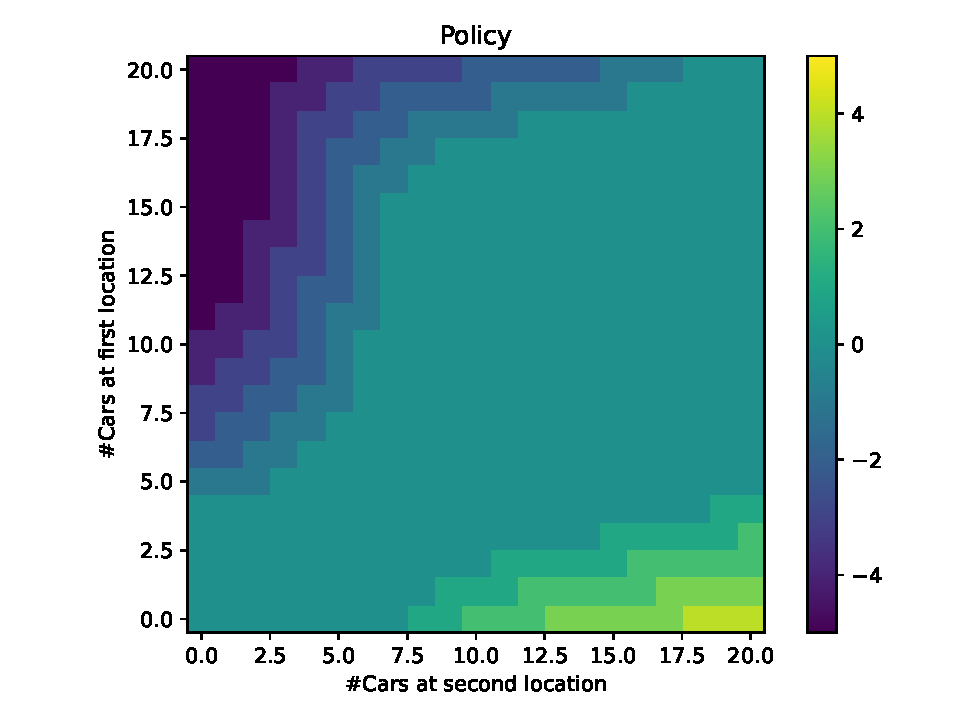
\includegraphics[width=0.8\textwidth]{chapters_latex/figures/ex_04_07_original.pdf}
    \caption{The original policy.}
\end{figure}

\begin{figure}[H]
    \centering
    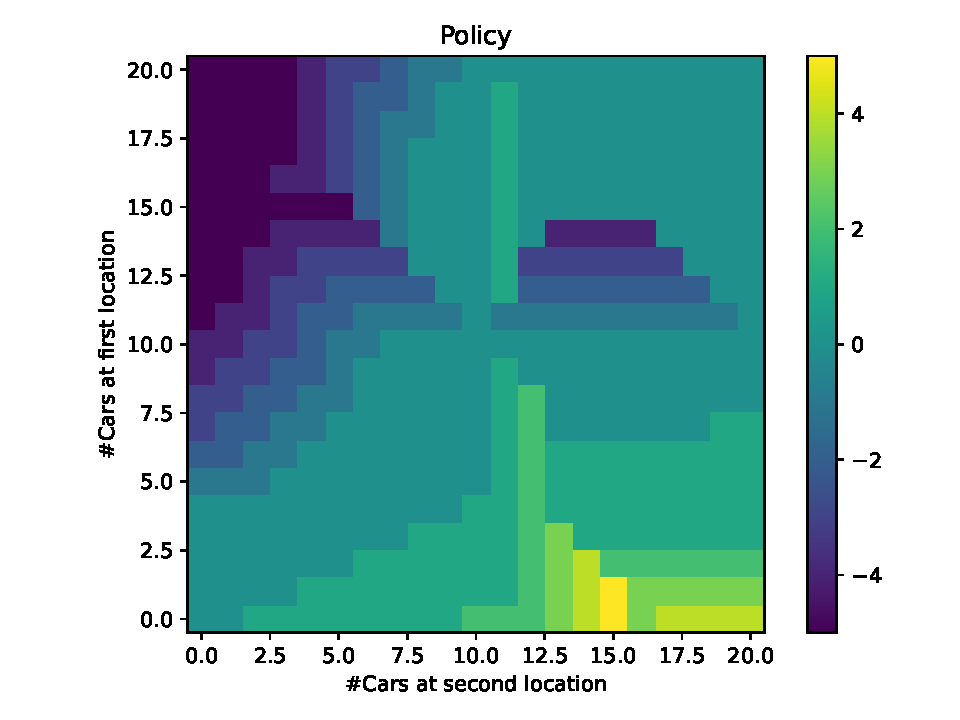
\includegraphics[width=0.8\textwidth]{chapters_latex/figures/ex_04_07_modified.pdf}
    \caption{The modified policy.}
\end{figure}

\subsection*{Exercise 4.8}
Why does the optimal policy for the gambler's problem have such a curious form? In particular, for capital of 50
it bets it all on one flip, but for capital of 51 it does not. Why is this a good policy? 

\subsubsection*{Solution:}

Betting 1 at 51 has two outcomes: receiving 1 coin with probability of 0.6 arriving at 52 coins, and losing 1 coin with probability of 0.4 arriving at 50 coins. At 50 coins we still have a relatively good chance of winning the game in one bet, and at 52 coins we have an even better chance. Betting more than one coin would mean that with great probability we would have less than 50 coins, in which case we would need a minimum of 2 bets to win the game, which is not good.

\subsection*{Exercise 4.9 (programming)}
Implement value iteration for the gambler's problem and
solve it for $p_h = 0.25$ and $p_h = 0.55$. In programming, you may find it convenient to
introduce two dummy states corresponding to termination with capital of 0 and 100,
giving them values of 0 and 1 respectively. Show your results graphically, as in Figure 4.3.
Are your results stable as $\theta \rightarrow 0$?

\subsubsection*{Solution:}

See the notebooks.

The state values for different head probabilities:

\begin{figure}[H]
    \centering
    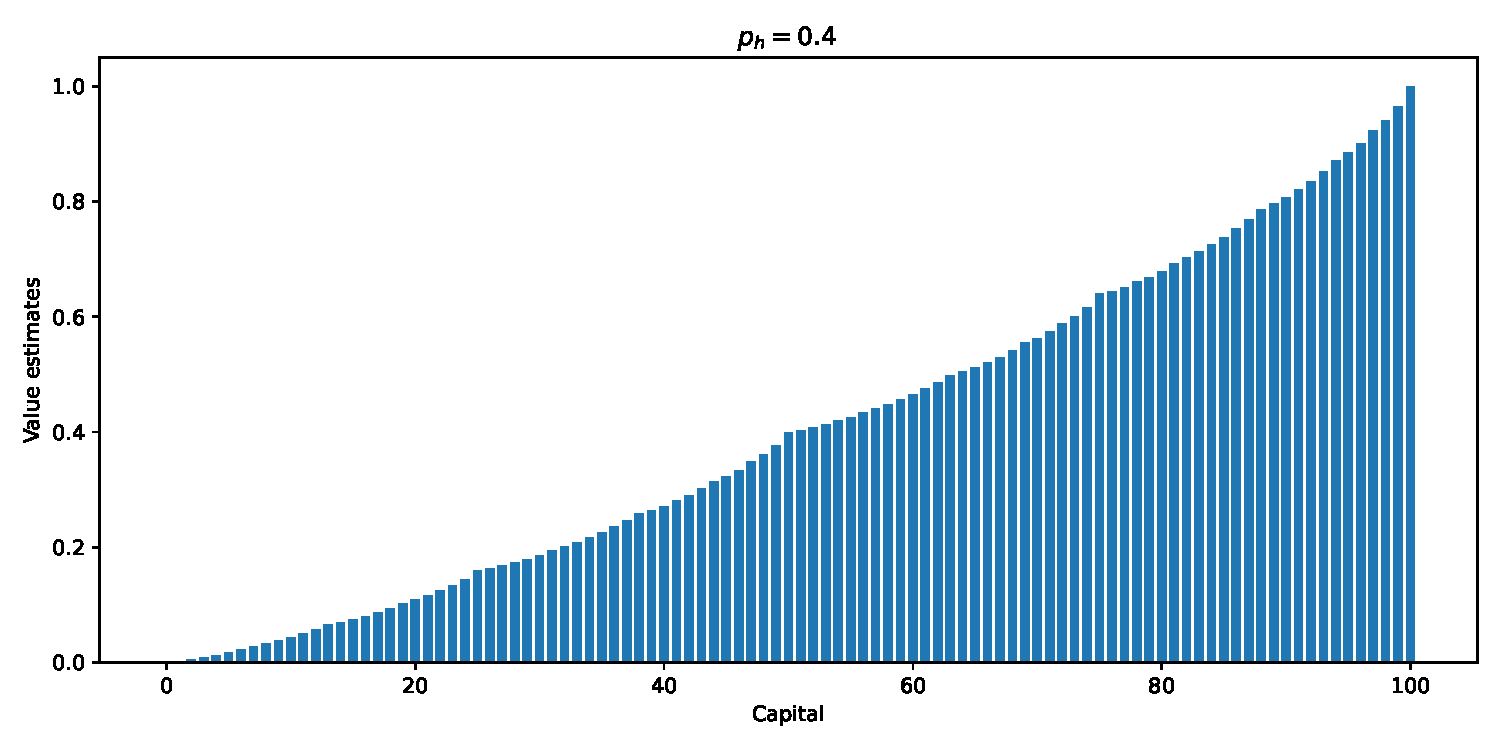
\includegraphics[width=0.8\textwidth]{chapters_latex/figures/ex_04_09_values_04.pdf}
\end{figure}

\begin{figure}[H]
    \centering
    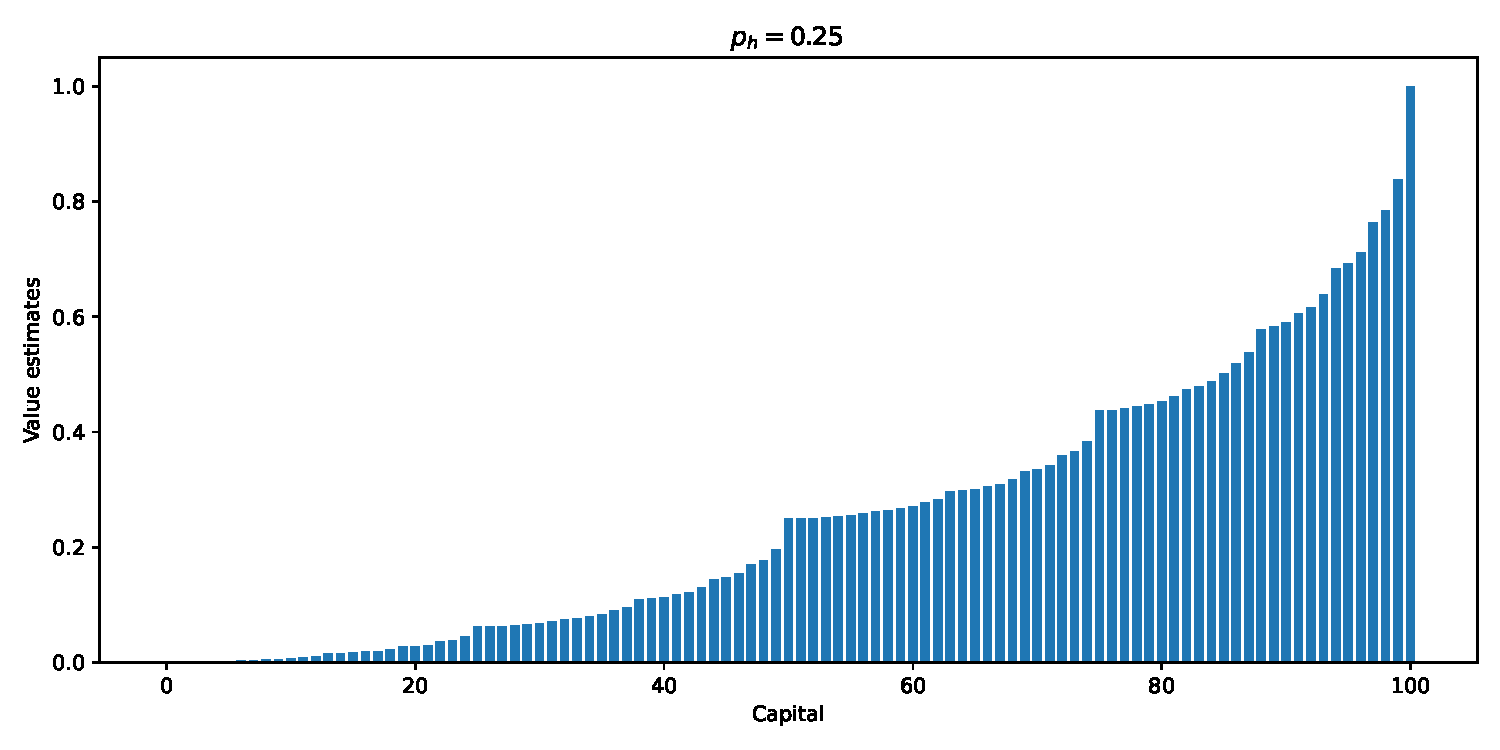
\includegraphics[width=0.8\textwidth]{chapters_latex/figures/ex_04_09_values_025.pdf}
\end{figure}

\begin{figure}[H]
    \centering
    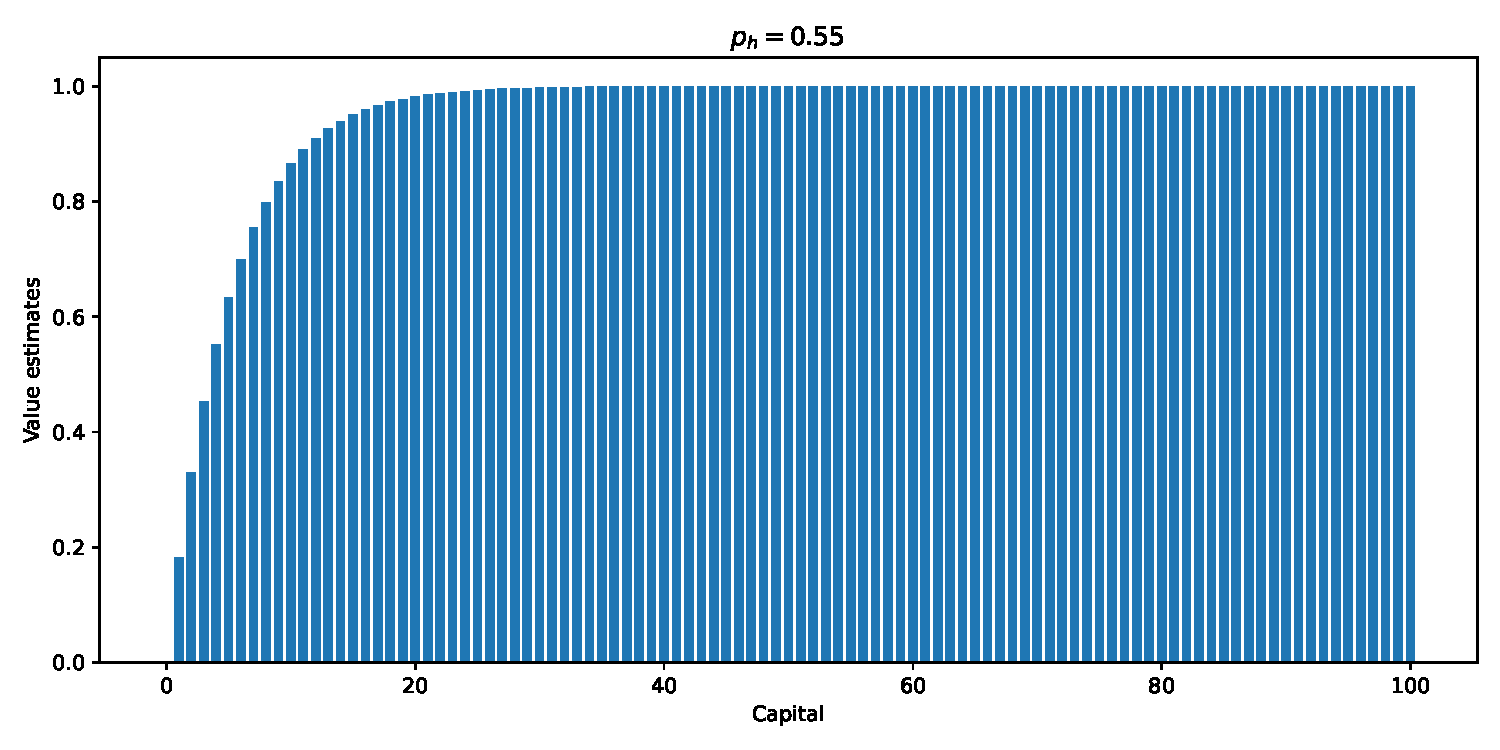
\includegraphics[width=0.8\textwidth]{chapters_latex/figures/ex_04_09_values_055.pdf}
\end{figure}

The optimal policies for different head probabilities:
\begin{figure}[H]
    \centering
    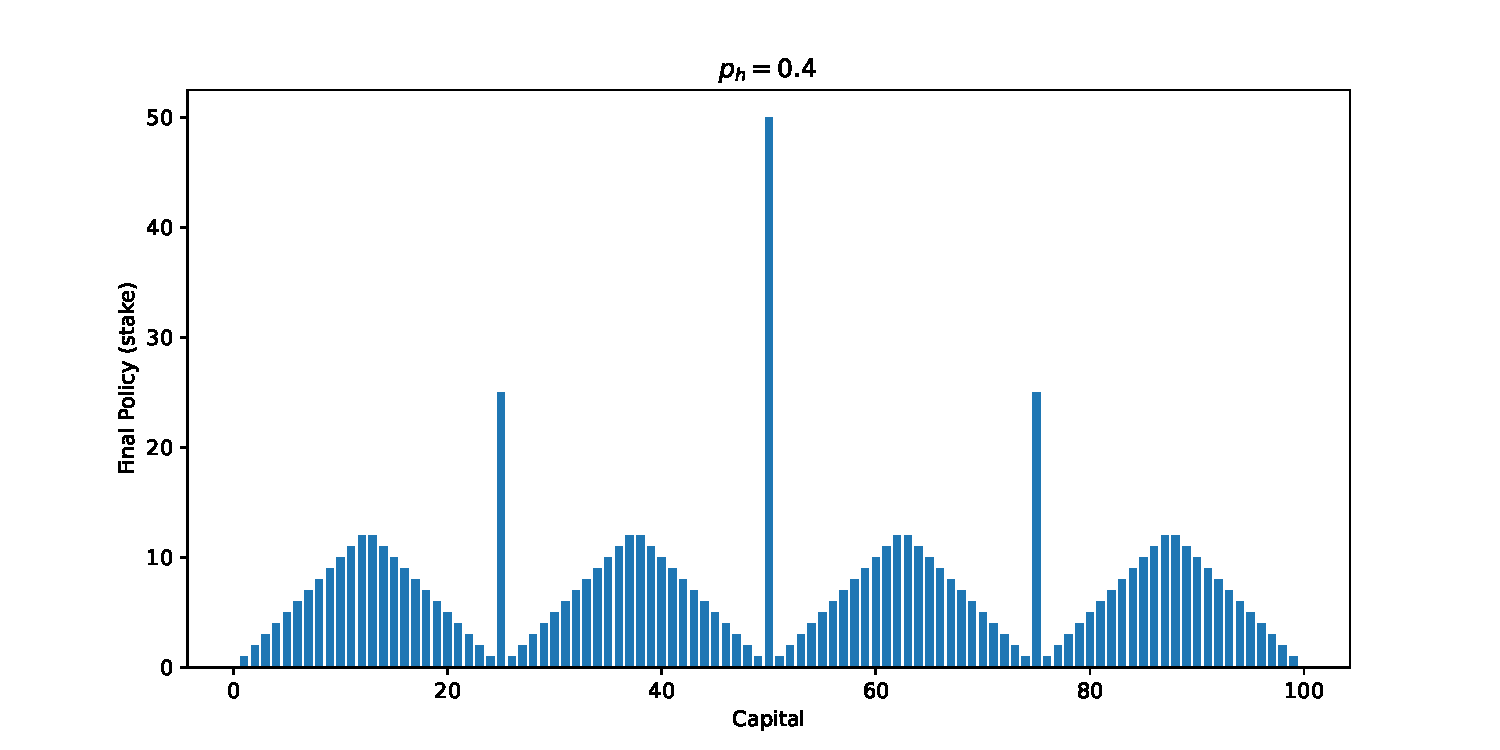
\includegraphics[width=0.8\textwidth]{chapters_latex/figures/ex_04_09_policies_04.pdf}
\end{figure}

\begin{figure}[H]
    \centering
    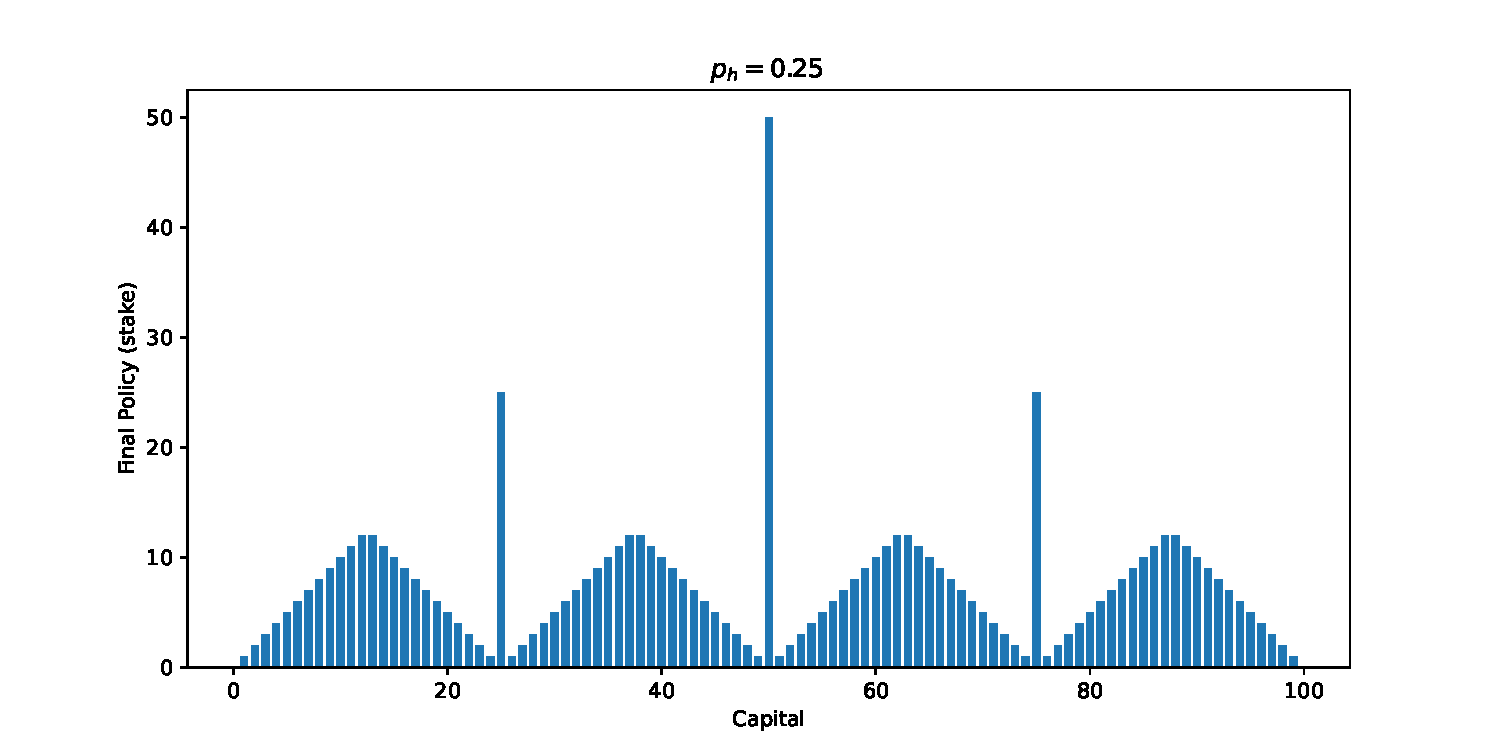
\includegraphics[width=0.8\textwidth]{chapters_latex/figures/ex_04_09_policies_025.pdf}
\end{figure}

\begin{figure}[H]
    \centering
    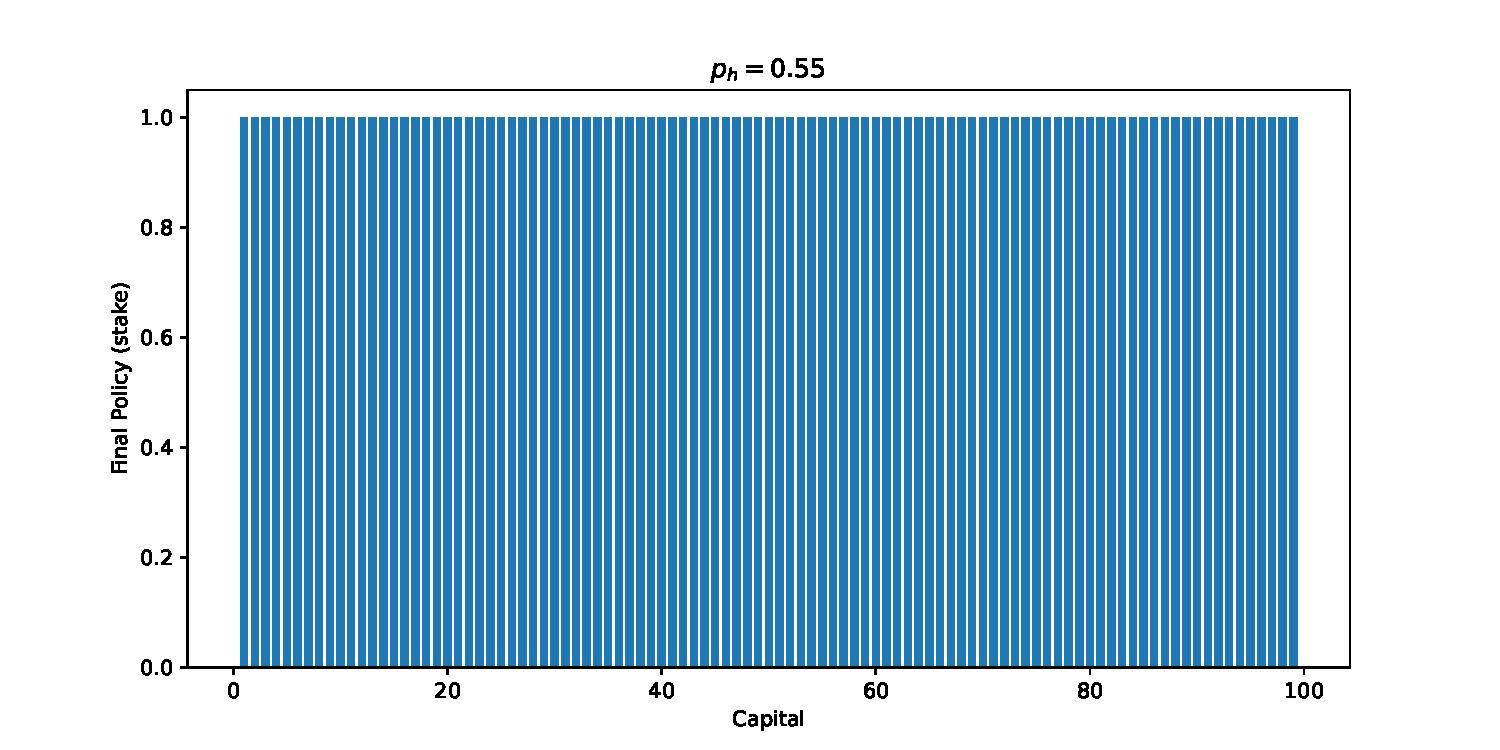
\includegraphics[width=0.8\textwidth]{chapters_latex/figures/ex_04_09_policies_055.pdf}
\end{figure}

\subsection*{Exercise 4.10}

What is the analog of the value iteration update (4.10) for action values,
$q_{k+1}(s,a)$?

\subsubsection*{Solution:}
\[
    q_{k+1}(s,a) = \sum_{s,r'} p(s',r \mid s, a) \left[r + \gamma \max_{a'} q_{k}(s',a') \right]
\]